\subsection*{Choosing a different loading function}
When going from the simple case of the loading function being identically $1$, to it being a different function we need to evaluate the function in the point corresponding to the element we are in. For the whole matrix, the assignment is done by
\begin{align*}
	(B)_{i,j} = h^2\cdot f\Big(\frac{i}{N},\frac{j}{N}\Big) \quad \text{for } i,j = 1,...,N-1.
\end{align*}
In the parallel code, it is important to make sure that each node is able to map its elements to the correct corresponding points on the grid when evaluation the function $f$. This is done by using what we know about which, and how many, columns each node has.

\subsection*{Different boundary conditions}

So far, we have only considered homogenous Dirichlet boundary conditions. In the case of non-homogenous Dirichlet boundary conditions, the load matrix $\mathbf{B}$ would be different. Most of $\mathbf{B}$ would be as before, but the first and last rows and columns should contain the boundary point information from the discretization. \\
\\
We could have implemented the boundary condition in this way: each node gets the boundary value information, and apply the boundary conditions of the rows. Since it is known how many nodes the program uses, we can tell the first and the last node separately to apply the boundary conditions for the columns(for the first node it applies the boundary condition in the first column and the last node applies the boundary conditions in the last column).

\subsection*{Choosing a more complex domain}

We have also assumed that the domain is the unit square. If this was not the case, but we instead had had a rectangle with sides $L_x$ and $L_y$, i.e. $ \Omega = (0,L_x)\times (0,L_y)$, but still a regular finite grid with $(N+1)$ points in each spatial direction, we would have to use different values for the spacing, 
\begin{align*}
	h_x = \frac{L_x}{N} \quad \text{and} \quad h_y = \frac{L_y}{N}.
\end{align*}
In terms of the implementation, a few changes would have to be made. Because we still use a regular finite grid, $\mathbf{T}$ and $\mathbf{B}$ would still be $(N-1)\times (N-1)$ matrices, but now we cannot multiply the loading function with $h^2$ when creating the load matrix $\mathbf{B}$. The system \eqref{system2} would change to 
\begin{align*}
	\frac{1}{h_x^2}\mathbf{\Lambda\widetilde{U}} + \frac{1}{h_y^2}\mathbf{\widetilde{U}\Lambda} = \mathbf{\widetilde{B}}.
\end{align*}
Here, $\mathbf{\Lambda}$ and $\mathbf{\widetilde{U}}$ are the same as before, but $\mathbf{\widetilde{B}}$ is scaled with $\dfrac{1}{h^2}$. The calculation of $\mathbf{\widetilde{U}}^T$ would have to be done by
\begin{align*}
	\tilde{u}^T_{i,j} &= \frac{\tilde{b}^T_{i,j}}{\dfrac{\lambda_i}{h_x^2} + \dfrac{\lambda_j}{h_y^2}}, 1 \leq i, j \leq N-1.
\end{align*}
In total, the only things that would have to change in the implementation of the method, is the calculation of the load matrix $\mathbf{B}$ and the matrix $\mathbf{\widetilde{U}}^T$.

\subsection*{Possible bottlenecks}
Since we decide to split the matrix column wise and we have $2^k-1$ columns we'll (almost) never get a load balanced program. This way some processors must process $2^k-1$ more numbers than the others. It could be possible to split this in another way such that the processors share the load better. The computational difficulty of achieving this is however pretty big, but it probably could be done.
\\ \\
An obvious bottleneck is the bandwidth between the nodes in the system (as evidenced in figure \ref{fig:bestnodes}). Here we could have done some more testing. No matter the results of this, we think ordinary decency says that you should use all the computing power in the node you get access to and not to use any excess nodes because of a small performance boost. This bottleneck inspired us to do some more testing and the result is shown in figure \ref{fig:varynodes}.
\begin{figure}[h]
\centering
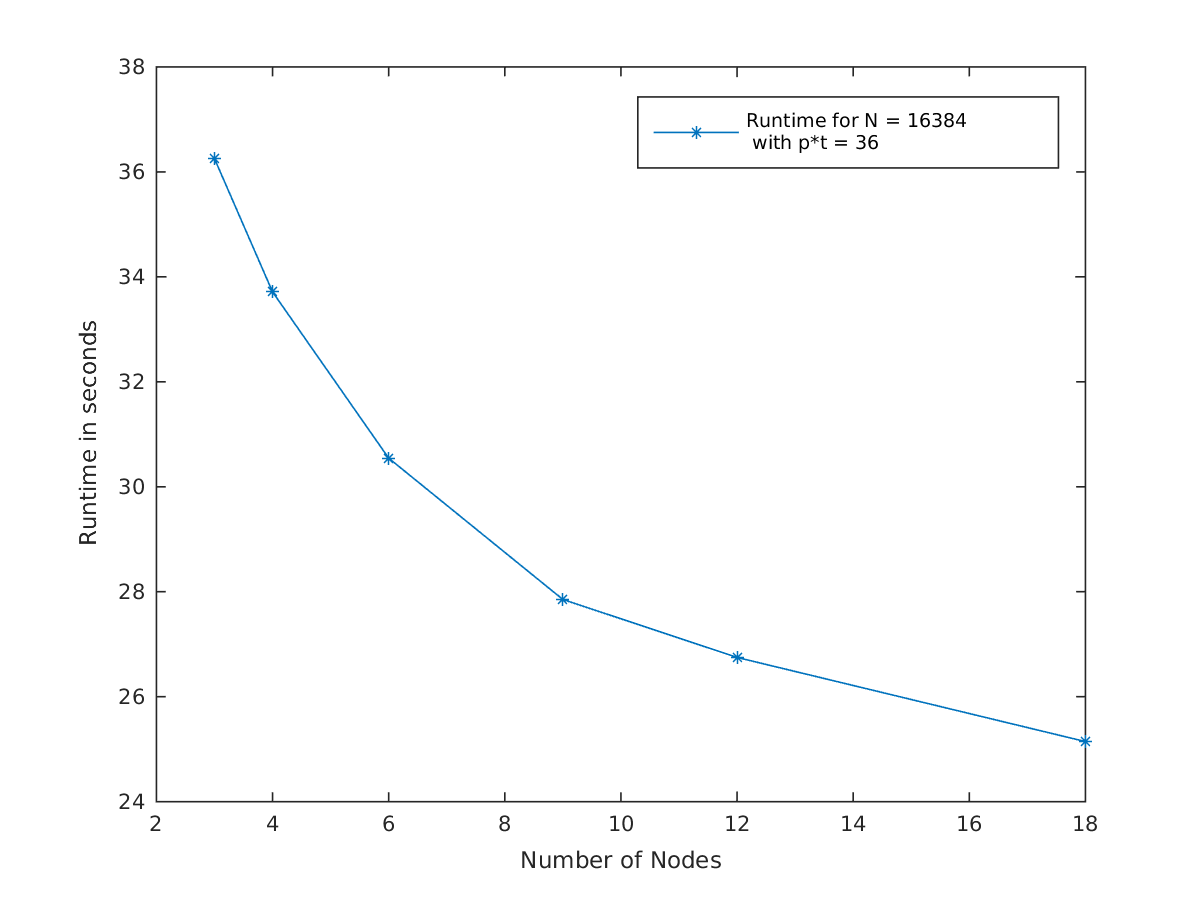
\includegraphics[width=0.7\textwidth]{./figures/varynodes}
\caption{Running the problem on a different amount of nodes with the combined number of processors to be 36 and each MPI core running on its own node ($n=p$).}
\label{fig:varynodes}
\end{figure}
As we can see we get a speedup when distributing the work over more nodes when $p\cdot t=36$. The best result here is also better than what we have already. We still feel like this is kind of like cheating, since we use so many nodes (without using them fully). It is however very effective and because of this we realize that the bandwidth is possible the most limiting bottleneck here.
\\ \\
If the resulting matrix should be stored, MPI-I/O could be used to store the matrix, but in our case we were only interested in whether or not it converged, so no need to store the data.
